\documentclass[a4paper, 12pt]{article}

\usepackage{hyperref}
\usepackage[warn]{mathtext}
\usepackage[utf8]{inputenc}
\usepackage[T2A]{fontenc}
\usepackage[english,russian]{babel}
\usepackage{multirow}
\usepackage{amsmath,amsfonts,amssymb,amsthm,mathtools}
\usepackage{indentfirst}
\DeclareSymbolFont{T2Aletters}{T2A}{cmr}{m}{it}
\usepackage{ gensymb }
\mathtoolsset{showonlyrefs=true}
\usepackage{euscript}
\usepackage{mathrsfs}
\usepackage[left=2cm,right=2cm,top=2cm,bottom=2cm]{geometry}
\usepackage{graphicx}
\usepackage{wrapfig}
\usepackage[rgb]{xcolor}
\hypersetup{
colorlinks=true,
urlcolor=blue
}
\usepackage{tikz}

\title{Лабораторная работа}
\author{Гисич Арсений Б03-102}
\date{2022}

\begin{document}

	\begin{center}
		{\large МОСКОВСКИЙ ФИЗИКО-ТЕХНИЧЕСКИЙ ИНСТИТУТ (НАЦИОНАЛЬНЫЙ ИССЛЕДОВАТЕЛЬСКИЙ УНИВЕРСИТЕТ)}
	\end{center}
	\vspace{5 cm}
	{\Large
		\begin{center}
			{\bf Лабораторная работа 3.2.3}\\[0.2 cm]
			Резонанс токов в параллельном контуре
		\end{center}
	}
	\vspace{4 cm}
	\begin{flushright}
		{\Large Выполнил: \\
			\vspace{0.2 cm}
			Гисич Арсений \\
			\vspace{0.2 cm}
			Б03-102 \\}
	\end{flushright}
	\vspace{9 cm}
	\begin{center}
		Долгопрудный\\[0.1 cm]
		2022
	\end{center}
\thispagestyle{empty}

\section{Аннотация}

В данной работе исследовался резонанс токов в параллельном колебательном контуре с изменяемой ёмкостью, были получены амплитудно-частотные и фазово-частотные характеристики, определены основные параметры контура.

\section{Теоретические сведения}

\begin{wrapfigure}{r}{0.3\textwidth}
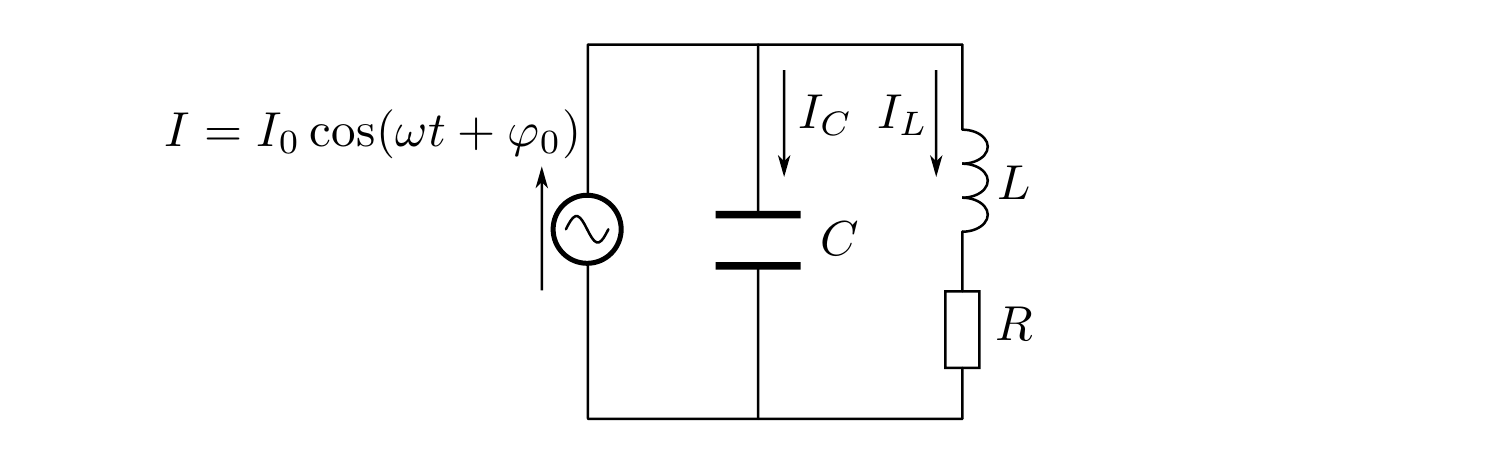
\includegraphics[width=0.3\textwidth]{1.png}
\caption{Последовательный контур с внешней ЭДС}
\label{r1}
\end{wrapfigure}

Рассмотрим процессы, протекающие в контуре, подключённом к источнику внешней ЭДС, изменяющейся по гармоническому закону $\varepsilon = \varepsilon_0 \cos{(\omega t + \varphi_0)}$. Для напряжения на конденсаторе $U_C(t)$ получим уравнение 
\begin{equation}\label{eq1}
\ddot{U}_C + 2\gamma \dot{U}_C + \omega_0^2U_С = \varepsilon_0\cos{(\omega t + \varphi_0)}.
\end{equation}

Перейдём к комплексному представлению колебаний. Запишем уравнение~\eqref{eq1} в комплексной форме, обозначая комплексные величины как <<векторы>>:
\begin{align}\label{eq2}
U_C & = \mathrm{Re}\,\mathbf{U_C}, & \mathbf{U_C} & = \mathrm{Re}\,\mathbf{U_C} + i\,\mathrm{Im}\,\mathbf{U_C}, \\
\varepsilon & = \mathrm{Re}\,\mathbf{\varepsilon}, & \mathbf{\varepsilon} & = \mathbf{\varepsilon_0}e^{i\omega t} = \varepsilon_0e^{i(\omega t + \varphi_0)},
\end{align}
\begin{equation}\label{eq3}
\mathbf{\ddot{U}_C} + 2\gamma \mathbf{\dot{U}_C} + \omega_0^2\mathbf{U_С} = \omega_0^2\mathbf{\varepsilon}.
\end{equation}

Комплексный множитель $\mathbf{\varepsilon_0} = \varepsilon_0e^{i\varphi_0}$, стоящий перед $e^{i\omega t}$, называется \textit{комплексной амплитудой}.

Решив уравнение~\eqref{eq3}, получим комплескное выражение для напряжения на конденсаторе $\mathbf{U_C}$. \textit{Вещественная часть} этого решения $\mathrm{Re}\,\mathbf{U_C}$ и является решением исходного уравнения~\eqref{eq1}. Будем искать решение уравнения~\eqref{eq3} в виде
\begin{equation}\label{eq4}
\mathbf{U_C}(t) = \mathbf{U_{C0}}e^{i\omega t},
\end{equation}
где $\mathbf{U_{C0}}$ --- комплексная амплитуда напряжения на конденсаторе, не зависящая от времени. Подставляя \eqref{eq4} в \eqref{eq3}, находим $\mathbf{U_{C0}}$ и далее, комплексные амплитуды тока в контуре и напряжений на сопротивлении и индуктивности:
\begin{equation}\label{eq5}
\mathbf{U_{C0}} = \frac{\mathbf{\varepsilon_0}}{i\omega CZ}, \quad Z = R + i\left(\omega L - \frac{1}{\omega C}\right),
\end{equation}
\begin{equation}\label{eq6}
\mathbf{I_0} = \frac{\mathbf{\varepsilon_0}}{Z}, \quad \mathbf{U_{R0}} = \frac{R\mathbf{\varepsilon_0}}{Z}, \quad \mathbf{U_{L0}} = i\omega L\frac{\mathbf{\varepsilon_0}}{Z}.
\end{equation}

Комплексная величина $Z$ называется \textit{комплексным сопротивлением}, или \textit{импедансом}, последовательного контура. Можно определить импеданс каждого отдельного элемента контура:
\begin{equation}\label{eq7}
Z_R = R, \quad Z_L = i\omega L, \quad Z_C = \frac{1}{i\omega C}.
\end{equation}

В новых обозначениях уравнения \eqref{eq5}--\eqref{eq6} принимают вид
\begin{equation}\label{eq8}
\mathbf{I} = \frac{\mathbf{\varepsilon_0}}{Z}, \quad \mathbf{U_{R0}} = Z_R\mathbf{I_0}, \quad \mathbf{U_{C0}} = Z_C\mathbf{I_0}, \quad \mathbf{U_{L0}} = Z_L\mathbf{I_0}.
\end{equation}

Импеданс контура $Z$ не зависит от начальных условий, не содержит величин ни токов, ни напряжений, а определяется свойствами всех элементов, соединённых в контур, и частотой синусоидальной ЭДС, к которой он подключён. Таким образом, \textit{импеданс $Z$ является характеристикой колебательного контура на заданной частоте}.

Выражение \eqref{eq5} для импеданса контура $Z$ содержит действительную часть $$\mathrm{Re}\,Z = R,$$ называемую \textit{активным} сопротивлением контура, и мнимую часть $$\mathrm{Im}\,Z = \omega L - \frac{1}{\omega C},$$ носящую название \textit{реактивного} сопротивления.

Импедансы контура и его отдельных элементов --- комплексные числа --- могут быть представленны в показательной форме:
\begin{equation}\label{eq9}
Z = Z_0e^{i\psi},
\end{equation}
где $Z_0 = |Z|$ --- модуль комплексного числа, $\psi = \arg{Z}$ --- его аргумент (фаза). Для импеданса рассматриваемого последовательного контура при этом находим
\begin{equation}\label{eq10}
Z_0 = \sqrt{(\mathrm{Re}\,Z)^2 + (\mathrm{Im}\,Z)^2} = \sqrt{R^2 + \left(\omega L - \frac{1}{\omega C}\right)^2} = \frac{R}{\cos{\psi_I}},
\end{equation}
\begin{equation}\label{eq11}
\tan{\psi_I} = \frac{\mathrm{Im}\,Z}{\mathrm{Re}\,Z} = \frac{\omega L - \frac{1}{\omega C}}{R}.
\end{equation}
Ток в контуре и напряжения на отдельных его элементах теперь могут быть получены по формулам~\eqref{eq5}--\eqref{eq8}. Например, действительная часть тока в контуре
\begin{equation}\label{eq12}
I(t) = \frac{\varepsilon_0}{R}\cos{\psi_I}\cos({\omega t + \varphi_0 - \psi_I)}.
\end{equation}
Как видно из~\eqref{eq11}~и~\eqref{eq12}, угол~$\psi_I$, определяемый отношением мнимой и действительной частей импеданса, представляют собой сдвиг фаз между напряжением на последовательном контуре и током в нём, причём \textit{положительные значения угла~$\psi_I$ соответствуют отставанию фазы тока, а отрицательные --- опережению}. В общем случае, когда к источнику последовательно подключены резистор, конденсатор и катушка самоиндукции, сдвиг фазы $\psi_I$ лежит в пределах $-\pi/2 < \psi_I < \pi/2$.

\section{Методика измерений}

\begin{figure}[h!]
\begin{center}
    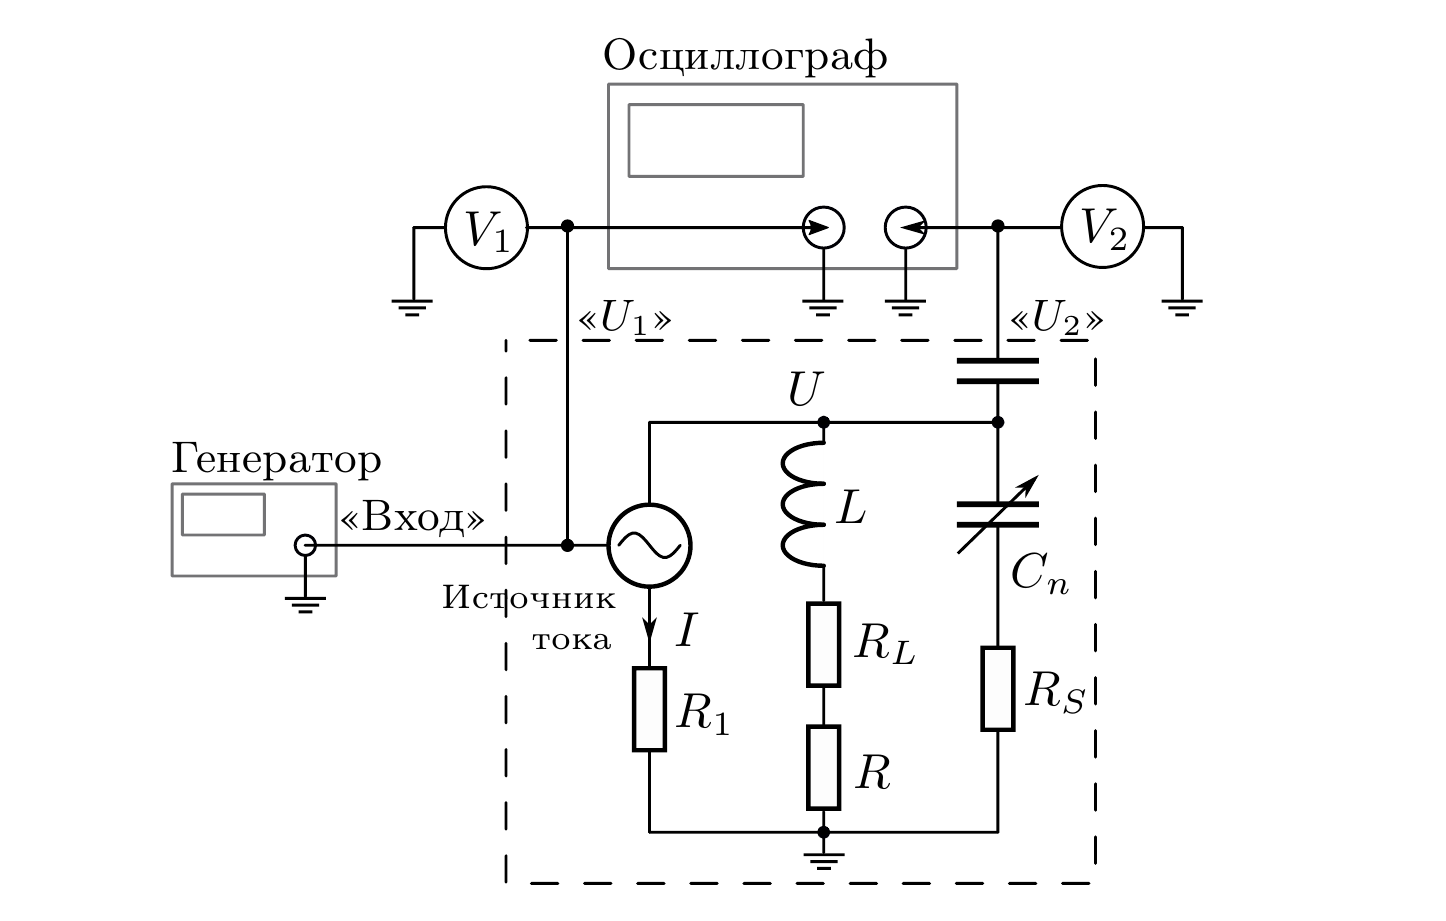
\includegraphics[scale=2.5]{ust.png}
\end{center}
\caption{Блок-схема экспериментального стенда}
\label{ust}
\end{figure}

$I=\dfrac{E}{R_I}=\dfrac{E_0cos(\omega t+\varphi_0)}{R_I}=I_0cos(\omega t+\varphi_0)$ --- ток на генераторе\newline
$$R_S=\dfrac{U_{RS}}{I}=\frac{U_{RS}}{\omega CU_{CS}}=\dfrac{1}{\omega C}tg\delta$$
где $R_S$ --- эквивалентное последовательное сопротивление (ЭПС)\newline
Для используемых емкостей $C_n$ выполнено $tg\delta<10^{-3}$\newline
$$R_{\sum}=R+R_L+R_S$$
где $R_{\sum}$ --- суммарное активное сопротивление контура.\newline
Воспользуемся методом комплексных амплитуд:\newline
$Z_L=R_L+i\omega L$, $Z_C=R_S-i\frac{1}{\omega C}$, $Z=R_{\sum}+i(\omega L-d\dfrac{1}{\omega C})$\newline
Тогда напряжение на контуре и токи на индуктивной и емкостной частях контура при нулевой начальной фазе можно представить в виде:\newline
$$I_c=I\dfrac{Z_L}{Z_C+Z_L}=iQI_0\dfrac{\omega}{\omega_0}\dfrac{1-i\dfrac{R+R_L}{\rho}\dfrac{\omega_0}{\omega}}{1+iQ(\dfrac{\omega}{\omega_0}-\dfrac{\omega_0}{\omega})}$$
$$I_L=I\dfrac{Z_c}{Z_C+Z_L}=iQI_0\frac{\omega_0}{\omega}\frac{1+itg\delta}{1+iQ(\frac{\omega}{\omega_0}-\frac{\omega_0}{\omega})}$$
$$U=I\frac{Z_LZ_c}{Z_C+Z_L}=Q\rho I_0\frac{(1-i\frac{R+R_L}{\rho}\frac{\omega_0}{\omega})(1+itg\delta)}{1+iQ(\frac{\omega}{\omega_0}-\frac{\omega_0}{\omega})}$$
где $\omega_0=\frac{1}{\sqrt{LC}}$ --- собственная частота, $\rho=\sqrt{\frac{L}{C}}$ --- реактивное сопротивление контура, $Q=\frac{\rho}{R_{\sum}}$ --- добротность контура\newline
Рассмотрим случай, когда $|\Delta\omega|=|\omega-\omega_0|\ll\omega_0$. Тогда
$$\frac{\omega}{\omega_0}-\frac{\omega_0}{\omega}=\frac{2\Delta\omega}{\omega_0}$$
Пренебрегая поправками порядка $Q^{-2}$, получим:
$$I_c=QI_0\frac{\omega}{\omega_0}\frac{e^{i\phi_c}}{\sqrt{1+(\tau\Delta\omega)^2}},    \phi_c=\frac{\pi}{2}-\frac{R+R_L}{\rho}-arctg(\tau\Delta\omega)$$
$$I_L=QI_0\frac{\omega_0}{\omega}\frac{e^{i\phi_L}}{\sqrt{1+(\tau\Delta\omega)^2}}, \phi_L=-\frac{\pi}{2}+\delta\arctg(\tau\Delta\omega)$$
$$U=Q\rho I_0\frac{\omega}{\omega_0}\frac{e^{i\phi_U}}{\sqrt{1+(\tau\Delta\omega)^2}}, \phi_U=-\frac{\omega}{\omega_0}\frac{R+R_L}{\rho}+\delta-arctg(\tau\Delta\omega)$$
где $\tau=\frac{2L}{R_{\sum}}=\frac{2Q}{\omega_0}$ --- время затухания.\newline
При резонансе, т.е. когда $\Delta\omega=0$:
$$I_c(\omega_0)=QI_0, \phi_c(\omega_0)=\frac{\pi}{2}-\frac{R+R_L}{\rho}$$
$$I_L(\omega_0)=QI_0, \phi_L(\omega_0)=-\frac{\pi}{2}+\delta$$
$$U(\omega_0)=Q\rho I_0=Q^2R_{\sum}I_0, \phi_U{\omega_0}=-\frac{R+R_L}{\rho}+\delta$$
$$\phi'_c(\omega_0)=\phi'_L(\omega_0)=\phi'_U(\omega_0)=-\tau$$
  	
\section{Используемое оборудование}

\begin{enumerate}
    \item генератор сигналов;
    \item источник напряжения;
    \item двухканальный осциллограф;
    \item цифровые вольтметры;
\end{enumerate}

\section{Результаты измерений и обработка данных}

Параметры установки:
\begin{description}
\item{} $R = 3,5~Ом$
\item{} $R_1 = 1008~Ом$
\end{description}

Результаты измерения резонансных частот для 7 разных конденсаторов и вычисления параметров контура представлены в таб.~\ref{tab1}. Параметры контура вычислим по формулам:

\begin{equation}
L=\frac{1}{C(2\pi f)^2} \\
\end{equation}
\begin{equation}
\rho=\frac{1}{2\pi fC} \\
\end{equation}
\begin{equation}
Z_{\text{рез}}=\frac{U}{E_0}R_1
\end{equation}
\begin{equation}
Q=\frac{UR_1}{E_0}2\pi fC
\end{equation}
\begin{equation}
R_{\sum}=\frac{E_0}{UR_1}\frac{1}{(2\pi fC)^2}
\end{equation}
\begin{equation}
R_{Smax}=10^{-3}\cdot\frac{1}{\omega_0C}
\end{equation}
\begin{equation}
R_L=\frac{E_0}{UR_1}\frac{1}{(2\pi fC)^2}-R-10^{-3}\cdot\frac{1}{\omega_0C}
\end{equation}

\begin{table}[h!]
\begin{center}
\begin{tabular}{|cccc|c|c|c|c|c|c|c|}
\hline
\multicolumn{1}{|c|}{$С, нФ$} & \multicolumn{1}{c|}{$f, кГц$} & \multicolumn{1}{c|}{$U, B$}  & $E, B$  & $L, мкГн$ & $\rho, Ом$ & $|Z_{рез}|, Ом$ & $Q$  & $R_{sum}, Ом$ & $R_{S_{max}}, Ом$ & $R_L, Ом$ \\ \hline
\multicolumn{1}{|c|}{25,1}  & \multicolumn{1}{c|}{32,12}  & \multicolumn{1}{c|}{1,190} & 0,202 & 978,2   & 197,4   & 5938,2     & 30 & 6,56     & 0,20      & 2,87     \\ \hline
\multicolumn{1}{|c|}{33,2}  & \multicolumn{1}{c|}{27,79}  & \multicolumn{1}{c|}{0,790} & 0,202 & 987,9   & 172,5   & 3942,2     & 23 & 7,55     & 0,17      & 3,88     \\ \hline
\multicolumn{1}{|c|}{47,3}  & \multicolumn{1}{c|}{23,16}  & \multicolumn{1}{c|}{0,670} & 0,202 & 998,4   & 145,3   & 3343,4     & 23 & 6,31     & 0,15      & 2,67     \\ \hline
\multicolumn{1}{|c|}{57,4}  & \multicolumn{1}{c|}{21,28}  & \multicolumn{1}{c|}{0,573} & 0,202 & 974,5   & 130,3   & 2859,3     & 22 & 5,94     & 0,13      & 2,31     \\ \hline
\multicolumn{1}{|c|}{67,5}  & \multicolumn{1}{c|}{19,46}  & \multicolumn{1}{c|}{0,449} & 0,202 & 990,9   & 121,2   & 2240,6     & 18 & 6,55     & 0,12      & 2,93     \\ \hline
\multicolumn{1}{|c|}{82,7}  & \multicolumn{1}{c|}{17,67}  & \multicolumn{1}{c|}{0,380} & 0,202 & 981,0   & 108,9   & 1896,2     & 17 & 6,26     & 0,11      & 2,65     \\ \hline
\multicolumn{1}{|c|}{101,6} & \multicolumn{1}{c|}{16,02}  & \multicolumn{1}{c|}{0,335} & 0,202 & 971,5   & 97,8    & 1671,7     & 17 & 5,72     & 0,10      & 2,12     \\ \hline
\multicolumn{4}{|c|}{Среднее значение}                                                         & 983,2   &         &            &    &          &           & 2,77     \\ \hline
\multicolumn{4}{|c|}{Случ. погрешность}                                                        & 3,6     &         &            &    &          &           & 0,21     \\ \hline
\end{tabular}
\end{center}
\caption{Параметры колебательного контура при разных значениях ёмкости конденсатора}
\label{tab1}
\end{table}

Результаты измерений амплитудно-частотной характеристики $U(\nu)$ для 1-ой ($25,1~нФ$) и 7-ой ($101,6~нФ$) ёмкостей конденсатора представлены в таб.~\ref{tab2}~и~\ref{tab3}.

\begin{table}[h!]
\begin{center}
\begin{tabular}{|c|c|c|c|}
\hline
$\nu, кГц$ & $\delta_{\nu}, кГц$ & $U, B$  & $\delta_U, B$ \\ \hline
31,38  & 0,01    & 0,682 & 0,001 \\ \hline
31,44  & 0,01    & 0,715 & 0,001 \\ \hline
31,51  & 0,01    & 0,765 & 0,001 \\ \hline
31,58  & 0,01    & 0,822 & 0,001 \\ \hline
31,69  & 0,01    & 0,910 & 0,001 \\ \hline
31,73  & 0,01    & 0,951 & 0,001 \\ \hline
31,78  & 0,01    & 0,992 & 0,001 \\ \hline
32,08  & 0,01    & 1,187 & 0,001 \\ \hline
32,86  & 0,01    & 0,705 & 0,001 \\ \hline
32,81  & 0,01    & 0,735 & 0,001 \\ \hline
32,68  & 0,01    & 0,825 & 0,001 \\ \hline
32,48  & 0,01    & 0,986 & 0,001 \\ \hline
32,30  & 0,01    & 1,127 & 0,001 \\ \hline
32,12  & 0,01    & 1,189 & 0,001 \\ \hline
\end{tabular}
\end{center}
\caption{Амплитудно-частотная характеристика колебательного контура для 1-ой ёмкости}
\label{tab2}
\end{table}

\begin{table}[h!]
\begin{center}
\begin{tabular}{|c|c|c|c|}
\hline
$\nu, кГц$ & $\delta_{\nu}, кГц$ & $U, B$  & $\delta_U, B$ \\ \hline
15,41  & 0,01    & 0,193 & 0,001 \\ \hline
15,51  & 0,01    & 0,215 & 0,001 \\ \hline
15,54  & 0,01    & 0,222 & 0,001 \\ \hline
15,60  & 0,01    & 0,239 & 0,001 \\ \hline
15,61  & 0,01    & 0,242 & 0,001 \\ \hline
15,64  & 0,01    & 0,250 & 0,001 \\ \hline
15,69  & 0,01    & 0,267 & 0,001 \\ \hline
15,78  & 0,01    & 0,289 & 0,001 \\ \hline
15,83  & 0,01    & 0,304 & 0,001 \\ \hline
15,92  & 0,01    & 0,325 & 0,001 \\ \hline
16,03  & 0,01    & 0,338 & 0,001 \\ \hline
16,71  & 0,01    & 0,200 & 0,001 \\ \hline
16,66  & 0,01    & 0,211 & 0,001 \\ \hline
16,60  & 0,01    & 0,223 & 0,001 \\ \hline
16,52  & 0,01    & 0,243 & 0,001 \\ \hline
16,44  & 0,01    & 0,264 & 0,001 \\ \hline
16,30  & 0,01    & 0,301 & 0,001 \\ \hline
16,15  & 0,01    & 0,332 & 0,001 \\ \hline
\end{tabular}
\end{center}
\caption{Амплитудно-частотная характеристика колебательного контура для 7-ой ёмкости}
\label{tab3}
\end{table}

График амплитудно-частотных характеристик $U(\nu)$ для обеих ёмкостей представлен на рис.~\ref{plot1}.

\begin{figure}[h!]
\begin{center}
    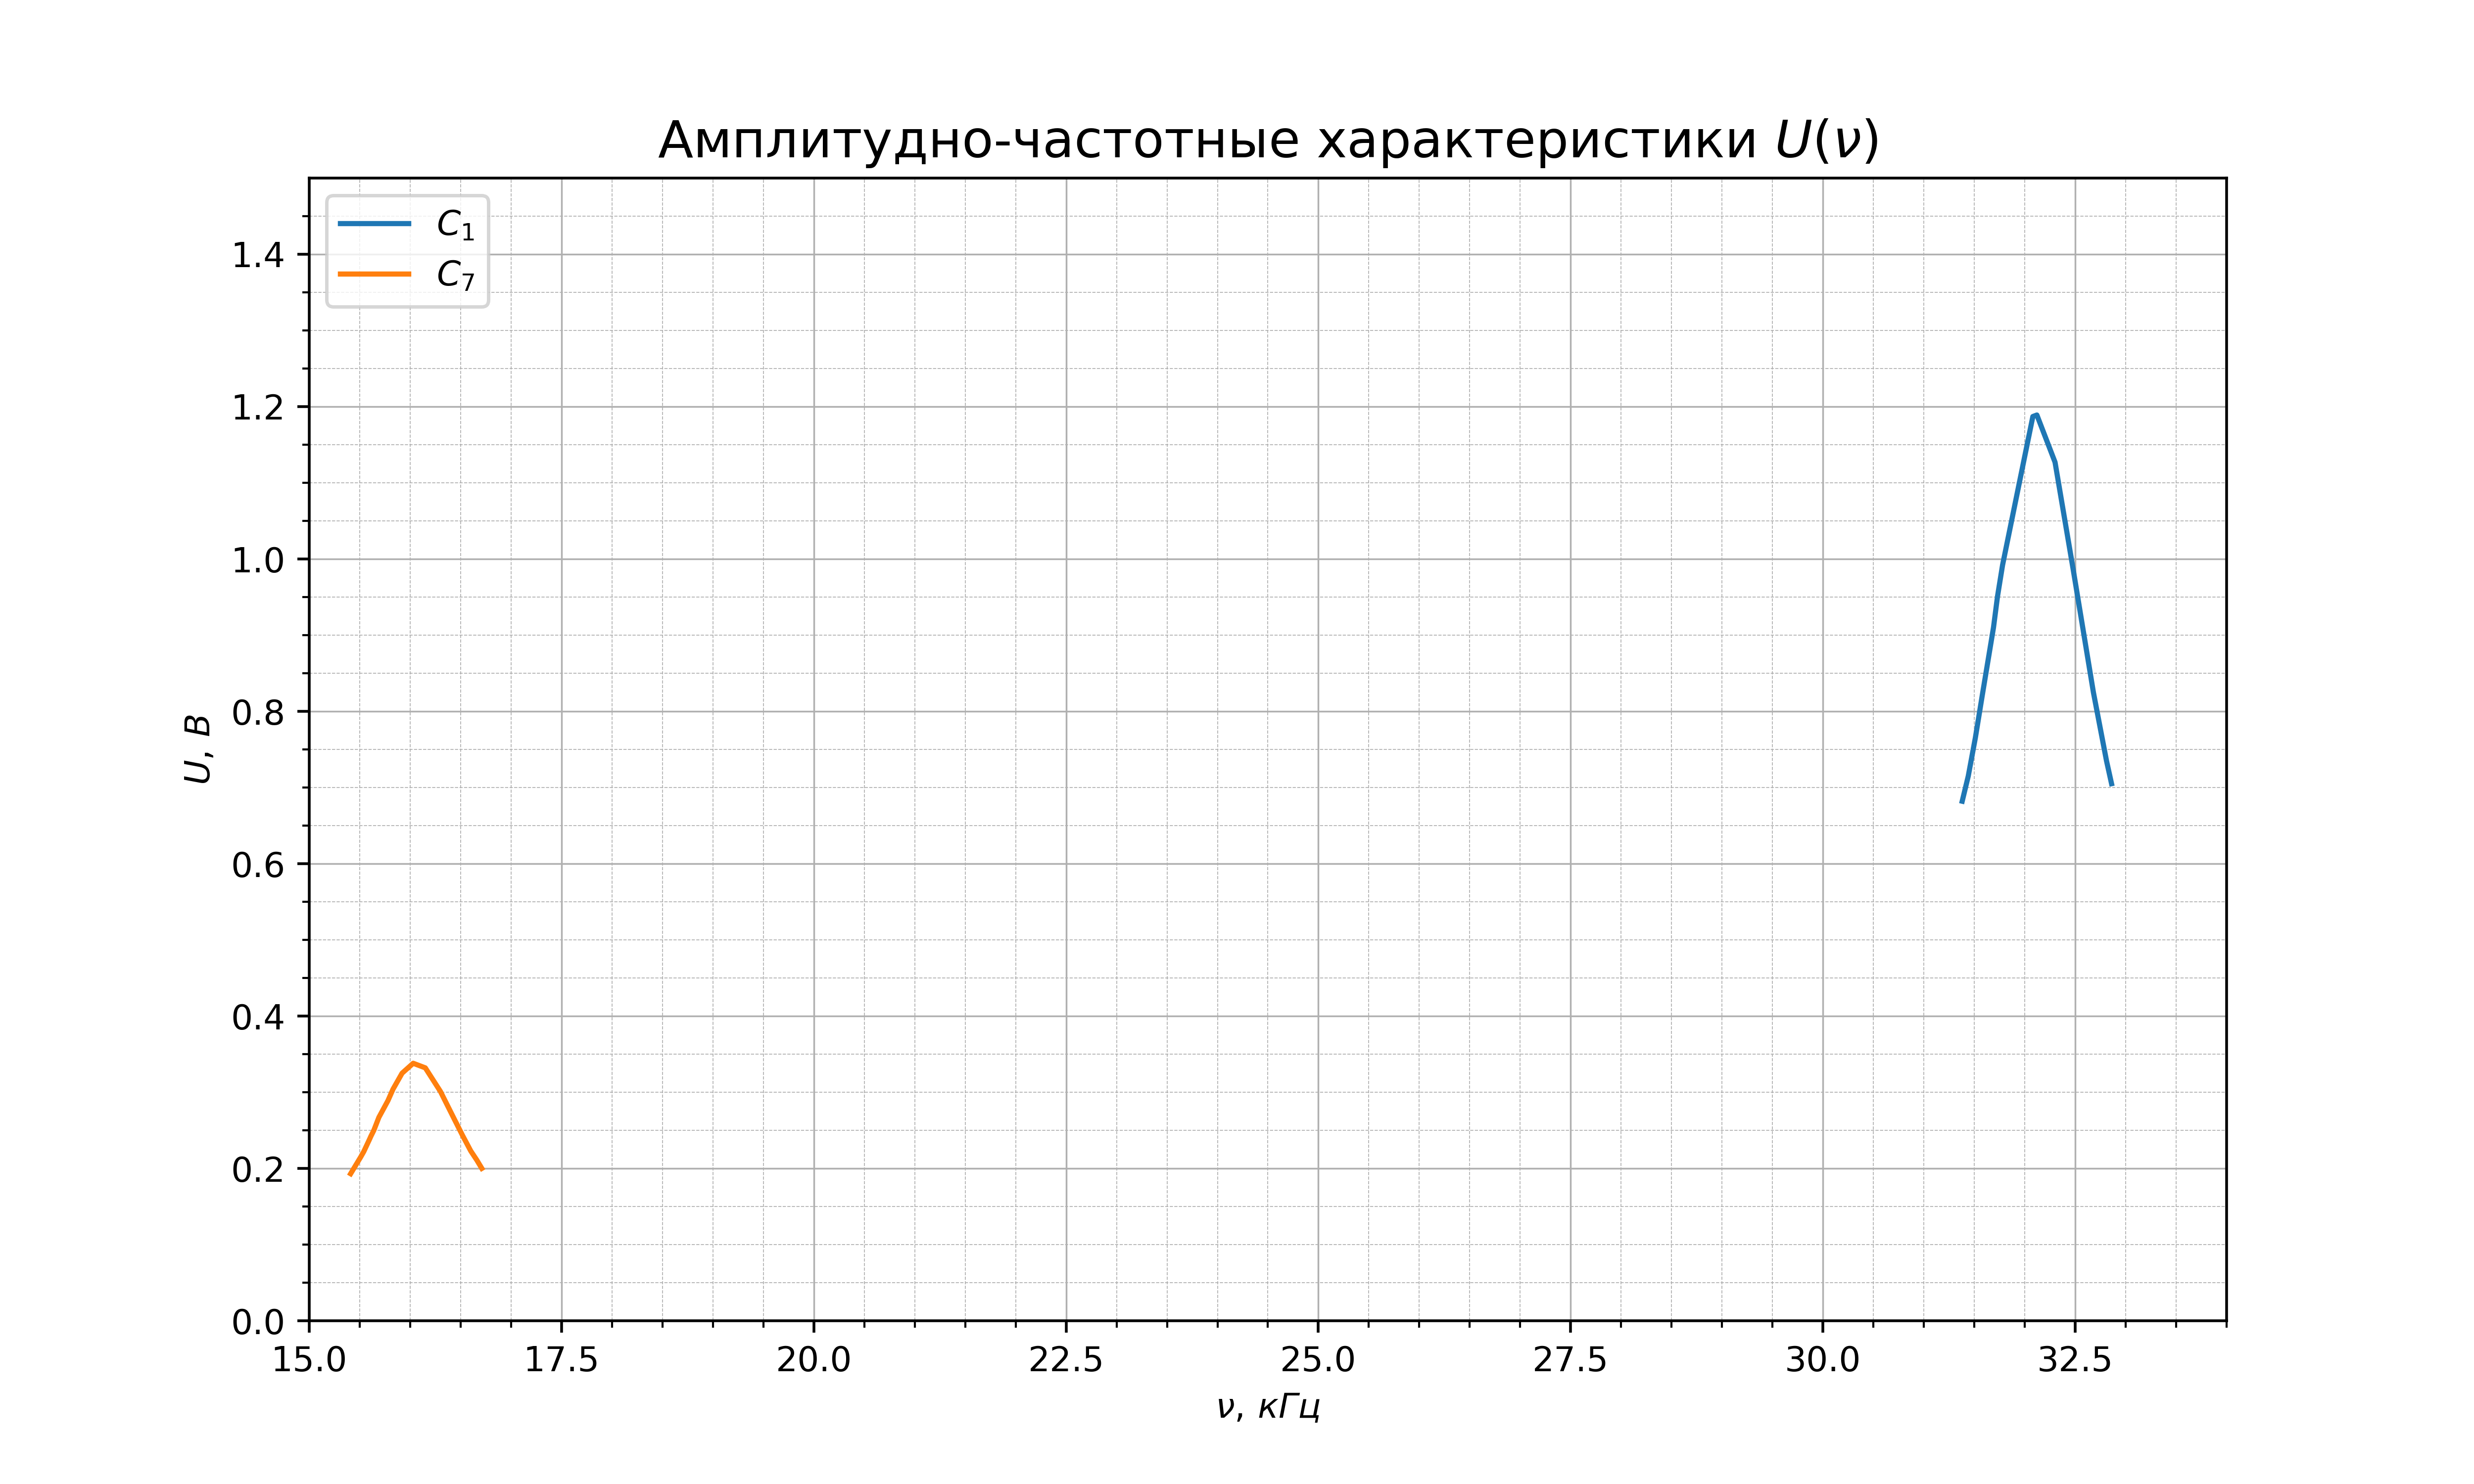
\includegraphics[scale=0.7]{3.2.3_1.png}
\end{center}
\caption{Амплитудно-частотная характеристика $U(\nu)$ для колебательного контура с 1-ой и 7-ой ёмкостями конденсатора}
\label{plot1}
\end{figure}

\newpage

График амплитудно-частотных характеристик $U(\nu)$ для обеих ёмкостей в безразмерных координатах представлен на рис.~\ref{plot2}. Кривая для ёмкости $C_7$ шире, чем для ёмкости $C_1$, что говорит о меньшей добротности контура с ёмкостью $C_7$.

\begin{figure}[h!]
\begin{center}
    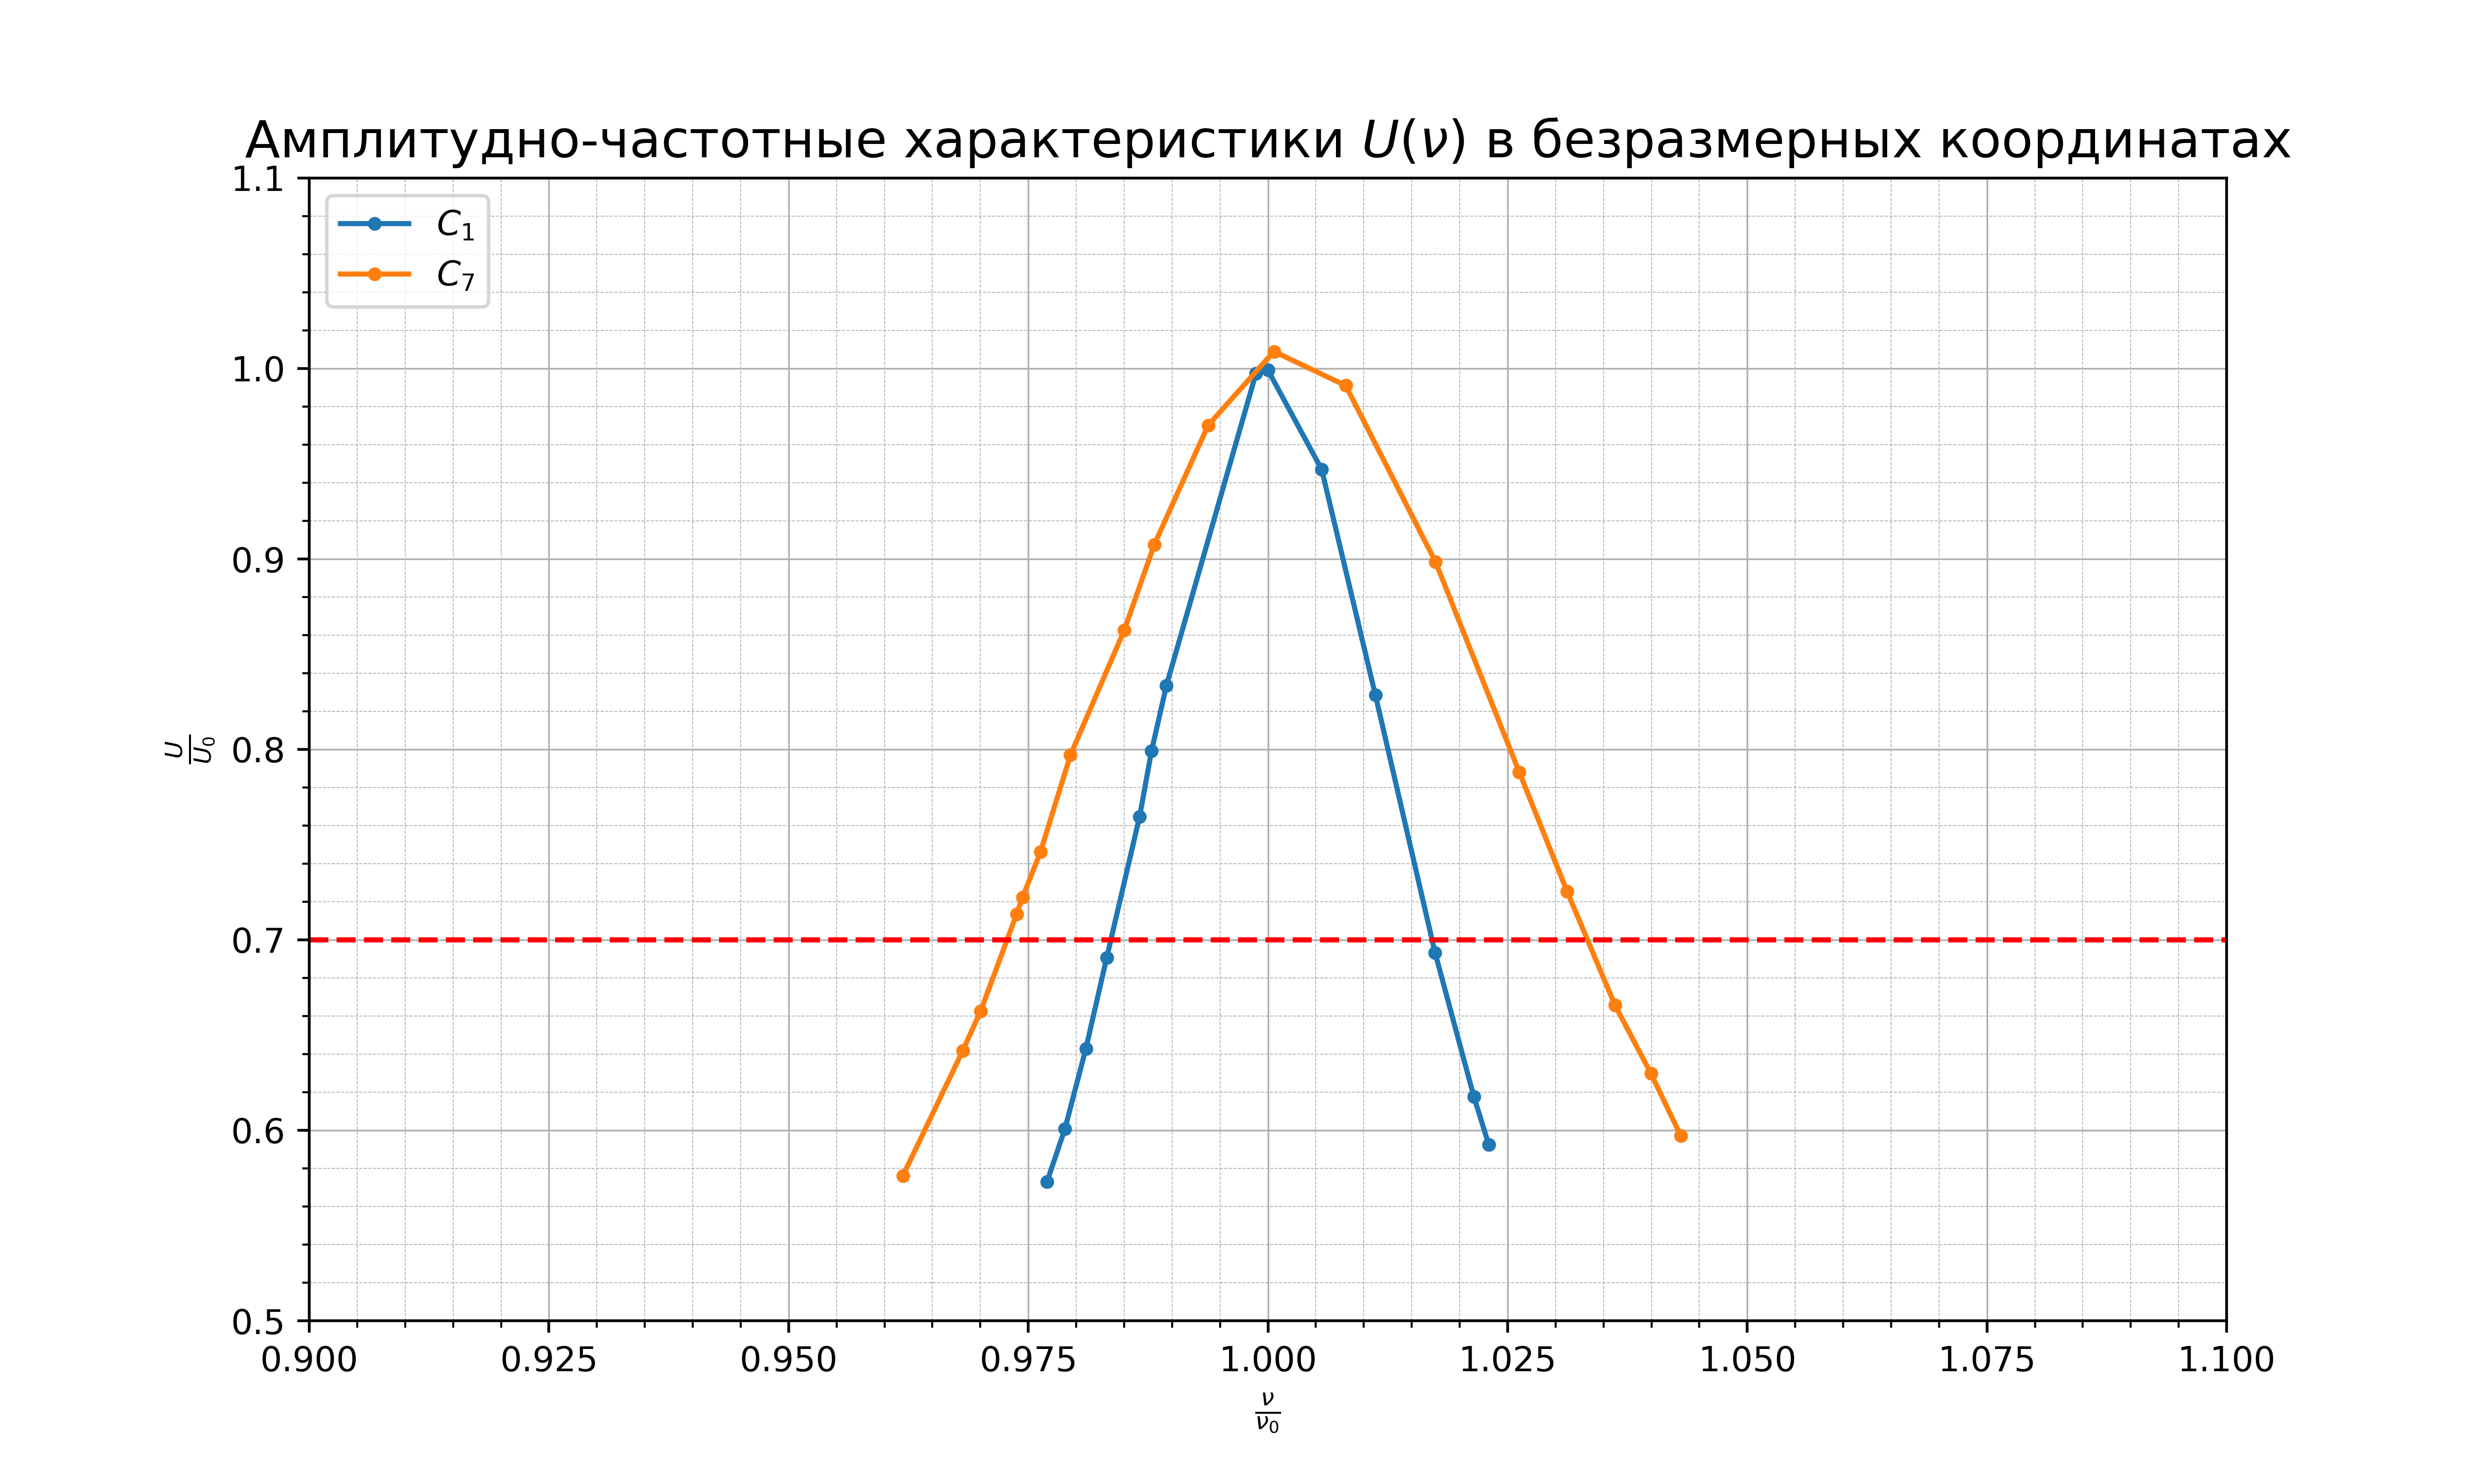
\includegraphics[scale=0.7]{3.2.3_2.png}
\end{center}
\caption{Амплитудно-частотная характеристика $U(\nu)$ для колебательного контура с 1-ой и 7-ой ёмкостями конденсатора в безразмерных координатах}
\label{plot2}
\end{figure}

Добротность определяется по формуле $Q = \frac{1}{\delta \omega}$, где $\delta \omega$ --- ширина резонансных кривых на уровне $\frac{1}{\sqrt{2}} = 0,707$. Полученные значения добротности:
$$ Q_1 = 29\pm1, \quad Q_7 = 16\pm1.$$

\newpage

Результаты измерений фазово-частотной характеристики $\psi_U(\nu)$ для 1-ой и 7-ой ёмкостей конденсатора представлены в таб.~\ref{tab4}~и~\ref{tab5}.

\begin{table}[h!]
\begin{center}
\begin{tabular}{|c|c|c|c|c|c|c|c|c|}
\hline
$\nu, кГц$ & $\delta_{\nu}, кГц$ & знак $\psi_U$ & $x, дел$ & $\delta_x, дел$ & $x_0, дел$ & $\delta_{x_0}, дел$ & $\psi_U, \pi \cdot рад$ & $\delta_{\psi_U}, \pi \cdot рад$ \\ \hline
30,35  & 0,01    & -1         & 3,5    & 0,5     & 17,0    & 0,5      & -0,21        & 0,03           \\ \hline
30,75  & 0,01    & -1         & 3,5    & 0,5     & 17,0    & 0,5      & -0,21        & 0,03           \\ \hline
30,99  & 0,01    & -1         & 3,0    & 0,5     & 16,5    & 0,5      & -0,18        & 0,03           \\ \hline
31,10  & 0,01    & -1         & 3,0    & 0,5     & 16,5    & 0,5      & -0,18        & 0,03           \\ \hline
31,35  & 0,01    & -1         & 3,0    & 0,5     & 16,0    & 0,5      & -0,19        & 0,03           \\ \hline
31,56  & 0,01    & -1         & 2,0    & 0,5     & 16,0    & 0,5      & -0,13        & 0,03           \\ \hline
31,64  & 0,01    & -1         & 2,0    & 0,5     & 16,0    & 0,5      & -0,13        & 0,03           \\ \hline
31,88  & 0,01    & -1         & 0,5    & 0,5     & 16,0    & 0,5      & -0,03        & 0,03           \\ \hline
32,17  & 0,01    & 1          & 0,5    & 0,5     & 16,0    & 0,5      & 0,03         & 0,03            \\ \hline
32,50  & 0,01    & 1          & 3,0    & 0,5     & 16,0    & 0,5      & 0,19         & 0,03            \\ \hline
32,68  & 0,01    & 1          & 4,0    & 0,5     & 16,0    & 0,5      & 0,25         & 0,03            \\ \hline
32,81  & 0,01    & 1          & 4,5    & 0,5     & 16,0    & 0,5      & 0,28         & 0,03            \\ \hline
32,99  & 0,01    & 1          & 5,0    & 0,5     & 16,0    & 0,5      & 0,31         & 0,03            \\ \hline
33,21  & 0,01    & 1          & 5,0    & 0,5     & 15,5    & 0,5      & 0,32         & 0,03            \\ \hline
33,67  & 0,01    & 1          & 5,5    & 0,5     & 15,5    & 0,5      & 0,35         & 0,03            \\ \hline
34,28  & 0,01    & 1          & 6,5    & 0,5     & 15,0    & 0,5      & 0,43         & 0,04            \\ \hline
\end{tabular}
\end{center}
\caption{Фазово-частотная характеристика колебательного контура для 1-ой ёмкости}
\label{tab4}
\end{table}

\begin{table}[h!]
\begin{center}
\begin{tabular}{|c|c|c|c|c|c|c|c|c|}
\hline
$\nu, кГц$ & $\delta_{\nu}, кГц$ & знак $\psi_U$ & $x, дел$ & $\delta_x, дел$ & $x_0, дел$ & $\delta_{x_0}, дел$ & $\psi_U, \pi \cdot рад$ & $\delta_{\psi_U}, \pi \cdot рад$ \\ \hline
14,51  & 0,01    & -1         & 4,0    & 0,5     & 17,5    & 0,5      & -0,23        & 0,03           \\ \hline
14,90  & 0,01    & -1         & 4,0    & 0,5     & 17,0    & 0,5      & -0,24        & 0,03           \\ \hline
15,17  & 0,01    & -1         & 4,0    & 0,5     & 17,0    & 0,5      & -0,24        & 0,03           \\ \hline
15,51  & 0,01    & -1         & 3,5    & 0,5     & 16,5    & 0,5      & -0,21        & 0,03           \\ \hline
15,68  & 0,01    & -1         & 2,5    & 0,5     & 16,5    & 0,5      & -0,15        & 0,03           \\ \hline
15,82  & 0,01    & -1         & 2,0    & 0,5     & 16,0    & 0,5      & -0,13        & 0,03           \\ \hline
15,95  & 0,01    & -1         & 1,0    & 0,5     & 16,0    & 0,5      & -0,06        & 0,03           \\ \hline
16,12  & 0,01    & 1          & 0,5    & 0,5     & 16,0    & 0,5      & 0,03         & 0,03            \\ \hline
16,29  & 0,01    & 1          & 2,0    & 0,5     & 16,0    & 0,5      & 0,13         & 0,03            \\ \hline
16,46  & 0,01    & 1          & 4,0    & 0,5     & 16,0    & 0,5      & 0,25         & 0,03            \\ \hline
16,69  & 0,01    & 1          & 5,0    & 0,5     & 15,5    & 0,5      & 0,32         & 0,03            \\ \hline
17,02  & 0,01    & 1          & 5,5    & 0,5     & 15,0    & 0,5      & 0,37         & 0,04            \\ \hline
17,45  & 0,01    & 1          & 6,0    & 0,5     & 15,0    & 0,5      & 0,40         & 0,04            \\ \hline
\end{tabular}
\end{center}
\caption{Фазово-частотная характеристика колебательного контура для 7-ой ёмкости}
\label{tab5}
\end{table}

График фазово-частотных характеристик $\psi_U(\nu)$ для обеих ёмкостей в безразмерных координатах представлен на рис.~\ref{plot3}.

\begin{figure}[h!]
\begin{center}
    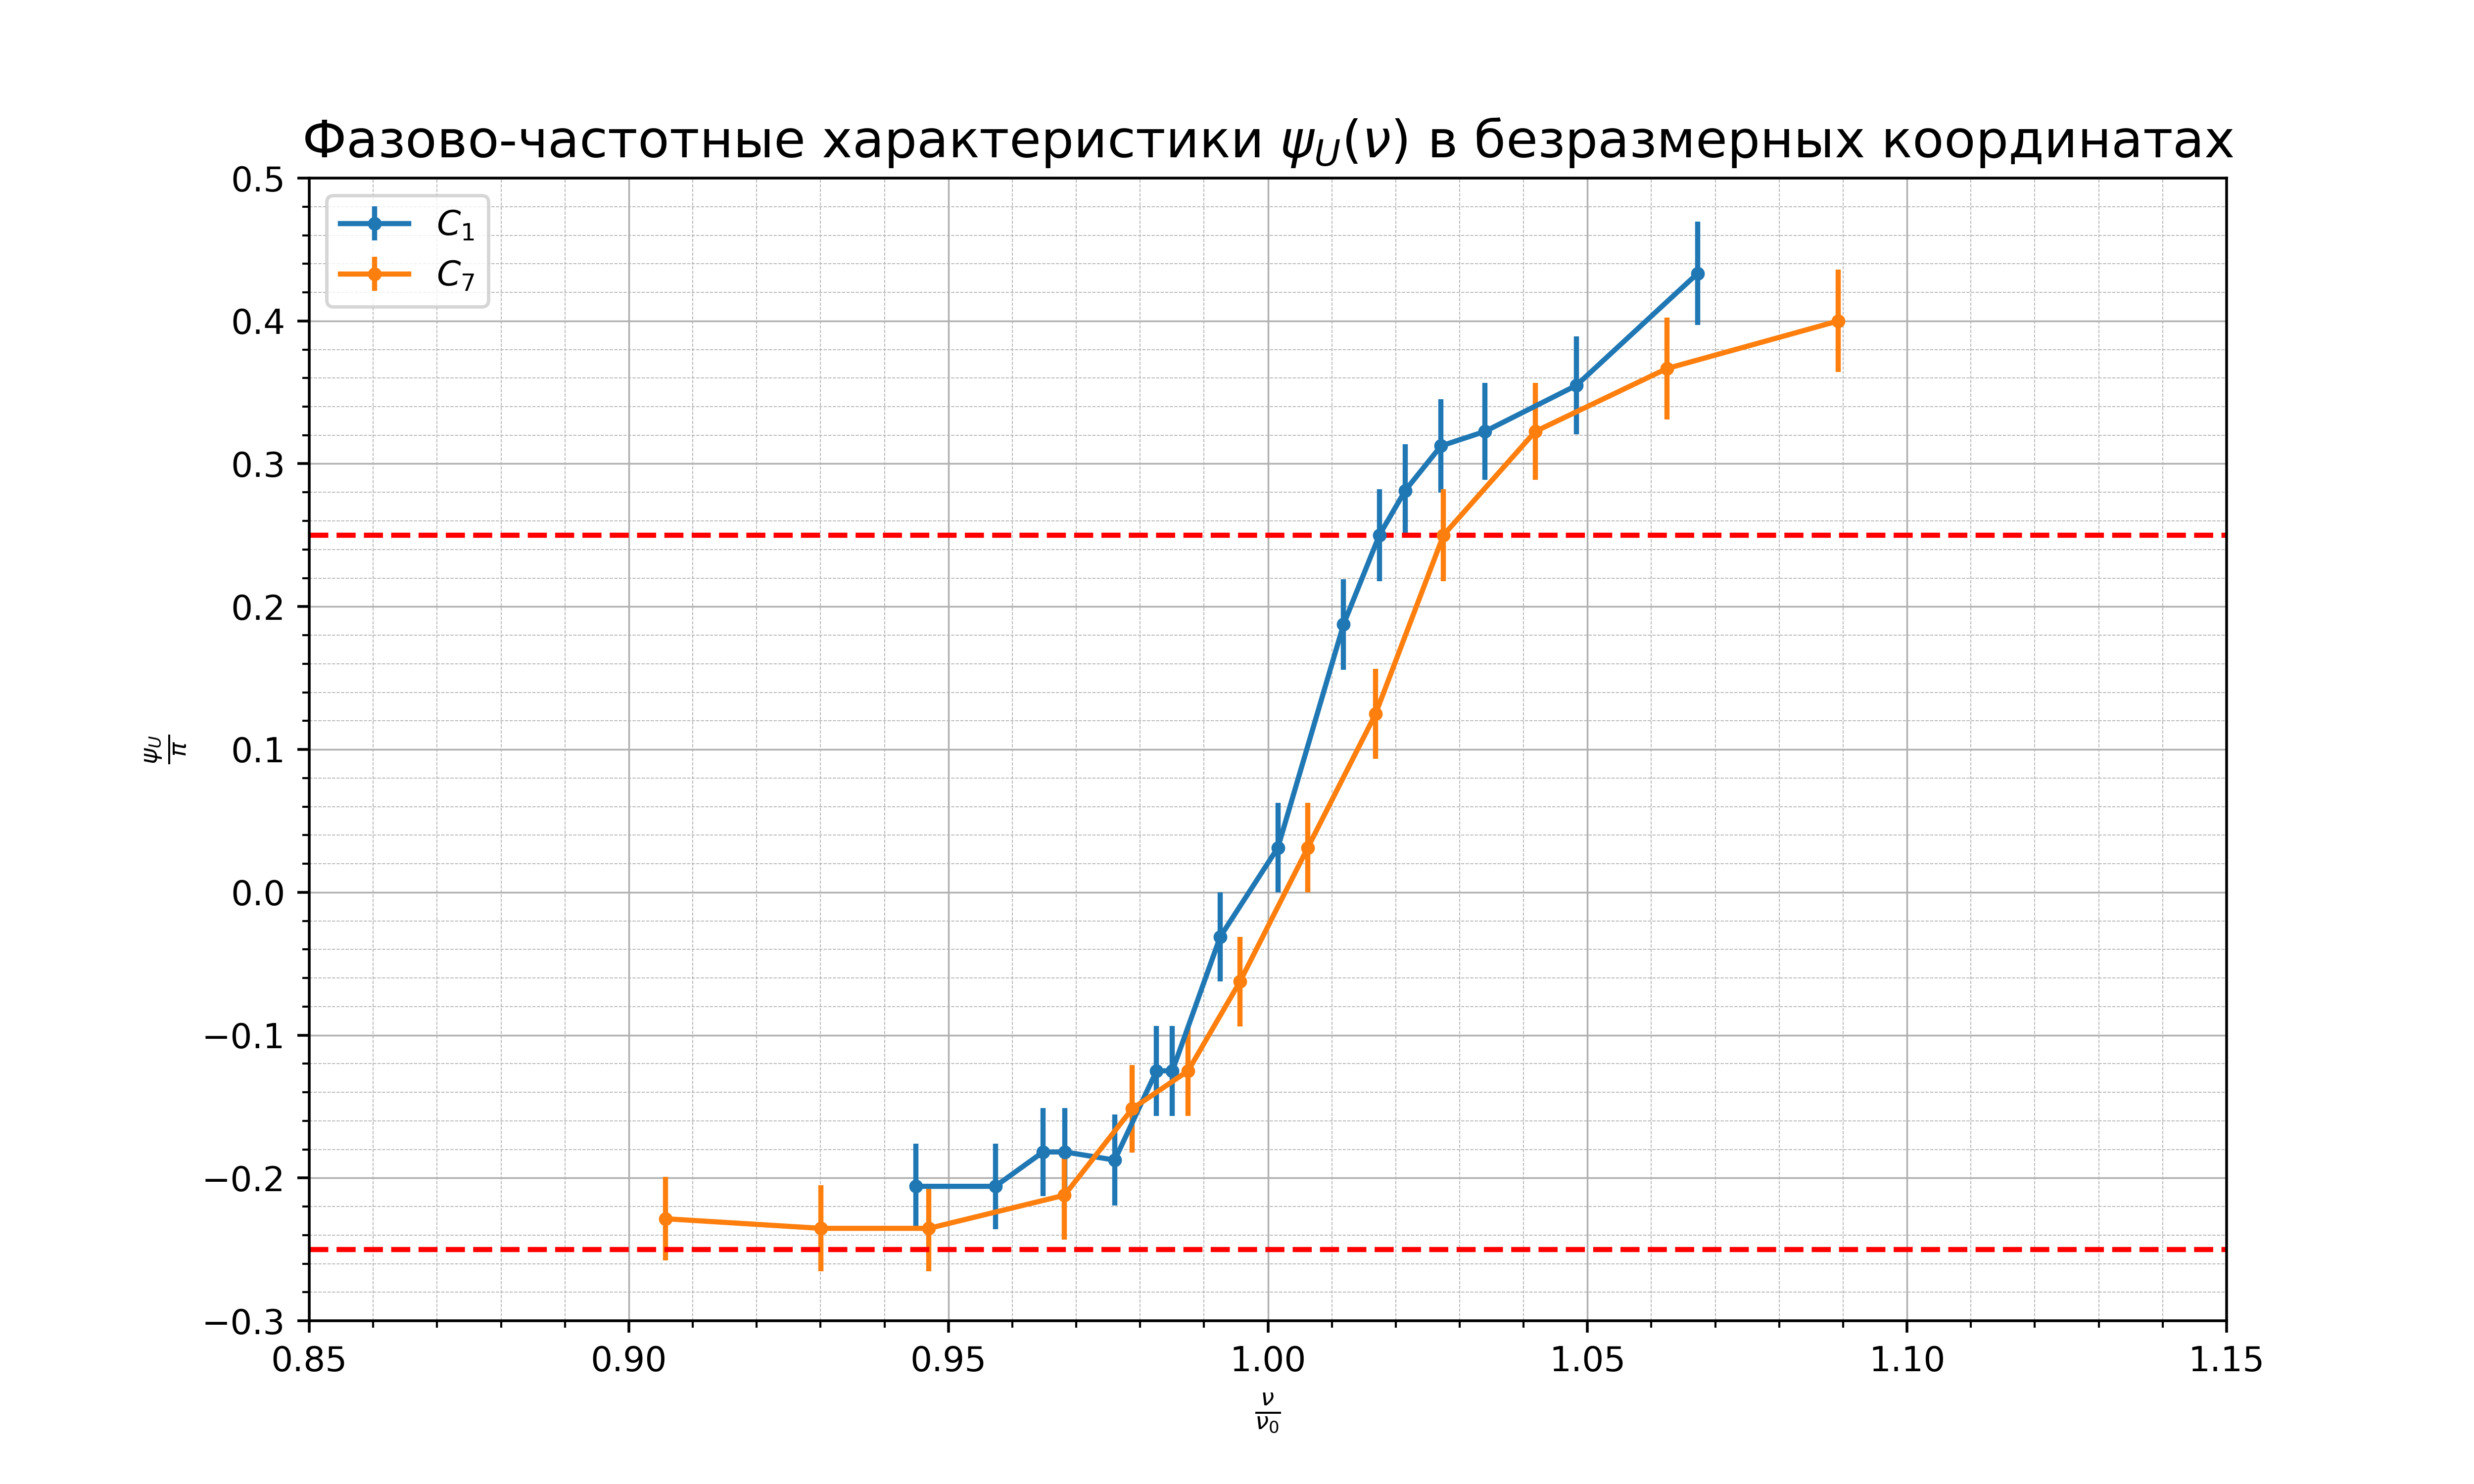
\includegraphics[scale=0.7]{3.2.3_3.png}
\end{center}
\caption{Фазово-частотная характеристика $\psi_U(\nu)$ для колебательного контура с 1-ой и 7-ой ёмкостями конденсатора в безразмерных координатах}
\label{plot3}
\end{figure}

Добротности контуров можно определить двумя способами: по формуле $Q = \frac{1}{2}\frac{d\psi_U(x)}{dx}$ при $x = 1$ или по расстоянию $1/Q$ между точками оси х, в которых y меняется от -1/4 до 1/4. Результаты измерения добротности 1-ым способом:
$$ Q_1 = 18\pm5, \quad Q_7 = 13\pm4.$$
Результаты измерения добротности 2-ым способом (так как график не доходит до -1/4, то были взяты значения, наиболее близкие к -1/4):
$$ Q_1 = 17\pm1, \quad Q_7 = 13\pm1.$$

График зависимости $R_L(\nu_{0n})$ представлен на рис.~\ref{plot4}.

\begin{figure}[h!]
\begin{center}
    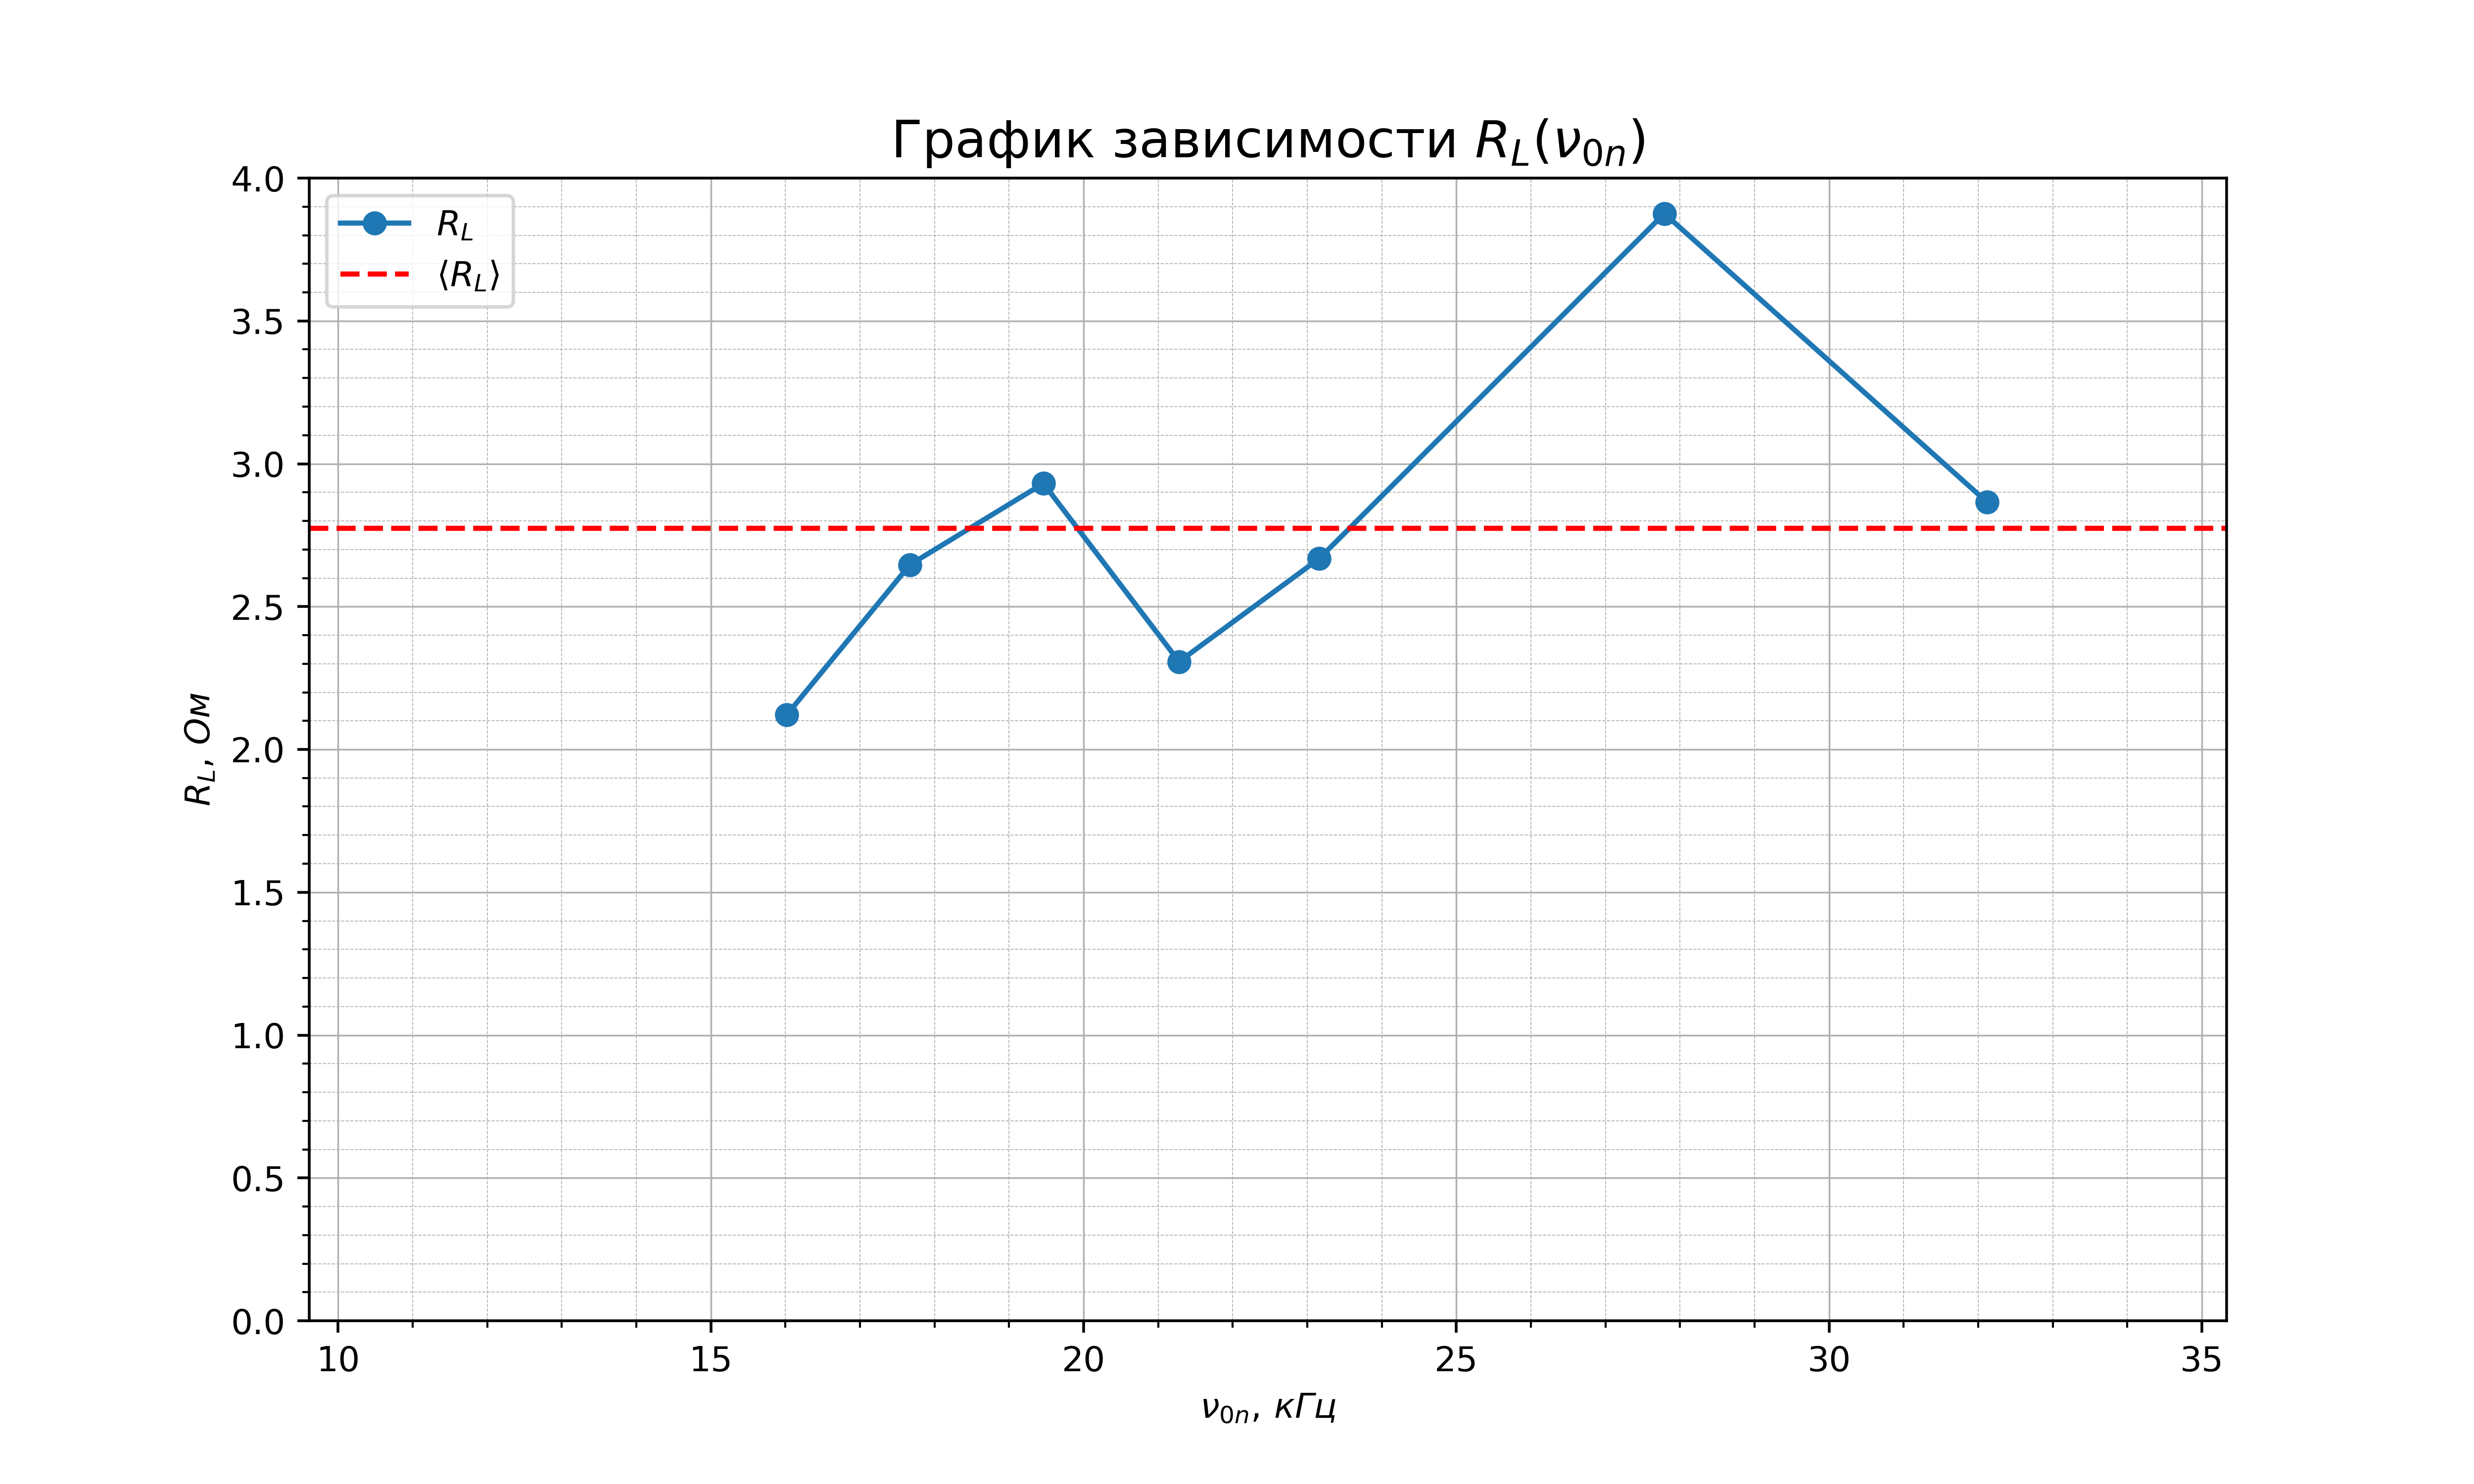
\includegraphics[scale=0.7]{3.2.3_4.png}
\end{center}
\caption{График зависимости активного сопротивления катушки $R_L$ от резонансной частоты контура $\nu_{0n}$}
\label{plot4}
\end{figure}

\newpage

\begin{wrapfigure}{l}{0.34\linewidth} 
	\begin{tikzpicture} [scale = 1.5, yshift=2pt]
		\draw  (0, 0) -- (0, 2.1);
		\draw (0, 0) -- (0, - 2.1);
		\draw  (0, 0) -- (2.5, 0);
		\draw [->] (0, 0) -- (0.75, 2) node[anchor=west] {$ \vec{I_C} $};
		\draw (0, 1.3) arc (60:0: 0.6);
			\draw (0.2,1.4) node {$ \varphi_C'$};
				\draw [->] (0, 0) -- (0.06, -2) node[anchor=west] {$ \vec{I_L} $};
			\draw (0, -1.3) arc (0:30: -0.4);
			\draw (0.15,-1.4) node {$ \delta$};
			\draw [->] (0, 0) -- (0.75, 0) node[anchor=south] {$ \vec{I} $};
			\draw [->] (0, 0) -- (1.75, -0.4) node[anchor=north] {$ \vec{U} $};
				\draw (1, 0) arc (30:0: 0.6);
					\draw (1.3, -0.1) node {$ \varphi_U$};
\end{tikzpicture}
\caption{Векторная диаграмма}
\end{wrapfigure}

Построим векторную диаграмму для контура с наименьшей добротностью, например, для $C_7$ с добротностью $Q_7 = 17$.

Посчитаем ток $ I = \dfrac{E}{R_1} = \dfrac{0,2}{1008} \approx 0,1 мА $. Его вектор равен сумме: $ \vec{I} = \vec{I_L} + \vec{I_C} $, причем $ \vec{I} $ расположен на оси абсцисс, а его компоненты расположены к нему под углами

\begin{equation}
\varphi_C = \dfrac{\pi}{2} - \dfrac{R + R_L}{\rho}, \quad \varphi_L = -\dfrac{\pi}{2} + \delta
\end{equation}

Здесь $ \delta \simeq 10^{-3}$ --- очень малый параметр установки, которым допустимо пренебречь при расчёте, однако можно изобразить для наглядности. Подсчитаем угол \newline $ \varphi_C' = \dfrac{R + R_L}{\rho} \approx 0,057 $. 

Аналогичный угол у напряжения $ \vec{U}: \varphi_U = - \dfrac{R + R_L}{\rho} $. Т.е. оно незначительно отклоняется от оси абсцисс на отрицательный угол.

\section{Обсуждение результатов и выводы}

В данной работе был исследован резонанс токов в параллельном колебательном контуре с изменяемой ёмкостью, были определены параметры контура, получены амплитудно-частотные и фазово-частотные характеристики контура при 2 различных значениях ёмкости конденсатора.  По графику АЧХ были определены добротности соответствующих контуров. Полученные значения:
$$ Q_1 = 29\pm1, \quad Q_7 = 16\pm1. $$
Также добротности были определены с помощью графика ФЧХ 2-мя способами. Значения, полученные 1-ым способом (по углу наклона прямой вблизи резонанса):
$$ Q_1 = 18\pm5, \quad Q_7 = 13\pm4. $$
Результат, полученный 2-ым способом (по расстоянию между y(-1/4) и y(1/4) по оси x):
$$ Q_1 = 17\pm1, \quad Q_7 = 13\pm1. $$
Значения добротности, рассчитанные теоретически:
$$ Q_1 = 30, \quad Q_7 = 17. $$
Результат, рассчитанный по АЧХ совпадает с теоретическим в пределах погрешности. Однако результаты, полученные при исследовании ФЧХ, совпадают по порядку, но существенно отличаются от рассчитанных теоретически. Это может быть связано с высокой погрешностью предложенного метода измерения сдвига фаз между $E$ и $U$ ввиду его сложности. Например, графики ФЧХ для обоих контуров не пересекают прямую $y = -1/4$, что говорит о наличии систематической погрешности измерений.

Также была определена зависимость активного сопротивления катушки $R_L$ от резонансной частоты $\nu_0$. Как видно из графика, $R_L$ возрастает с возрастанием частоты. Это может быть вызвано скин-эффектом. Резкое скачкообразное изменение значений $R_L$ может быть связано с изменением амплитуды ЭДС в процессе эксперимента.

\end{document}
